	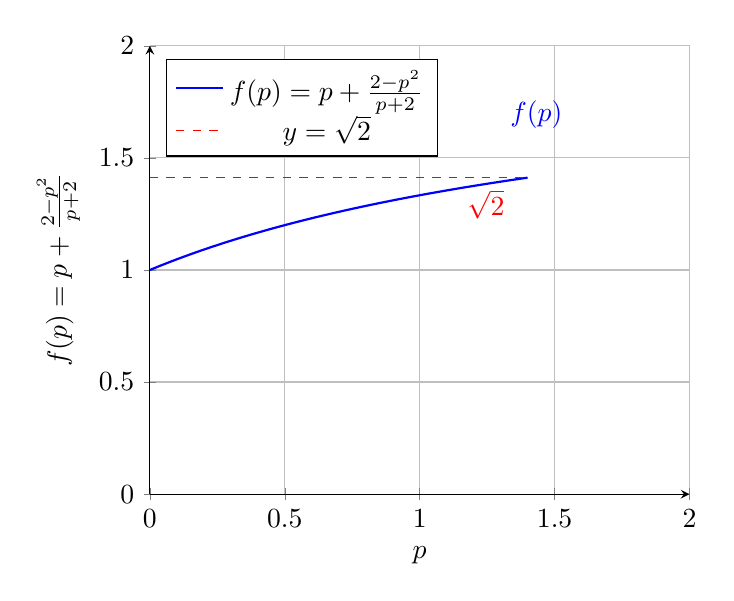
\begin{tikzpicture}
	\begin{axis}[
		axis lines = left,
		xlabel = {$p$},
		ylabel = {$f(p) = p + \frac{2 - p^2}{p + 2}$},
		xmin = 0, xmax = 2,
		ymin = 0, ymax = 2,
		domain = 0:1.4,
		samples = 100,
		legend pos = north west,
		grid = both,
		]
		% Plot the function f(m)
		\addplot[thick,blue,]
%		{x + (2 - x^2) / (x + 2)};
		{(2 * x + 2) / (x + 2)};
		\addlegendentry{$f(p) = p + \frac{2 - p^2}{p + 2}$}
		
		% Plot the horizontal line at y = sqrt(2)
		\addplot[dashed,red,]
		{sqrt(2)};
		\addlegendentry{$y = \sqrt{2}$}
		
		% Label points on the graph
		\node[below right, blue] at (axis cs:1.3,1.8) {$f(p)$};
		\node[below left, red] at (axis cs:1.35,1.4) {$\sqrt{2}$};
	\end{axis}
\end{tikzpicture}